% Full prose draft, October 30, 2026 (Chicago).
% Real-data results: validation-best checkpoints, comparisons/scores_valbest.csv
% (602 evaluations, completed October 18, 2026); inference: October 19 ANOVA.
% Exhibits: python papers/aaai27_relabeling/build_valbest_exhibits.py
\documentclass[letterpaper]{article}
\usepackage[submission]{aaai2027}
\usepackage[hyphens]{url}
\usepackage{graphicx}
\urlstyle{rm}
\def\UrlFont{\rm}
\usepackage{natbib}
\usepackage{caption}
\frenchspacing
\usepackage{booktabs}
\pdfinfo{/TemplateVersion (2027.1)}
\setcounter{secnumdepth}{2}
\title{Target Assignment in Synthetic Tabular Data}
\author{Anonymous Authors}
\affiliations{}
\begin{document}
\maketitle
\begin{abstract}
A synthetic training table needs both features and targets. Deep tabular
generators usually produce them together, but the target can instead be
assigned by a predictor trained on the real training data. We study this
choice as an experimental variable. For CTGAN, TVAE, and TabDDPM, we compare
three constructions: retaining generated targets, replacing the targets of
the same generated features with predictions from a real-data labeler, and
fitting a separate features-only generator before assigning predicted
targets. Across five classification and two regression tasks, two seeds,
synthetic-only and real-plus-synthetic training, and RF, XGBoost, and neural
labelers, predicted targets raise mean macro F1 by 7.4 percentage points in
synthetic-only training and 4.7 points in mixed training. The gains are
large for CTGAN, moderate for TVAE, and absent for TabDDPM, and neither
pooled effect survives multiplicity correction across five tasks. Whether
the generator sees the target before relabeling makes little measurable
difference. Seven simulated datasets with known distributions show
that relabeling consistently improves accuracy and agreement with the Bayes
rule, yet can worsen a density-refit measure of joint-distribution
fidelity. Target assignment should therefore be reported as a separate
design decision, and its predictive benefits should not be read as better
distributional fidelity.
\end{abstract}

\section{Introduction}
Synthetic tabular data are often judged by their \emph{utility}: a model
trained on synthetic rows is evaluated on held-out real rows. Most
generators used in this setting, including CTGAN and
TVAE~\citep{xu2019ctgan} and diffusion models such as
TabDDPM~\citep{kotelnikov2023tabddpm}, model the features $X$ and the target
$Y$ jointly. When downstream utility is the goal, however, the target column
plays a special role: it is the quantity the downstream model must learn,
and errors in the generated conditional $P(Y\mid X)$ translate directly into
label noise.

An alternative is to let the generator supply only the features and to
assign targets with a predictor $h$ trained on the real training set. This
resembles pseudo-labeling and knowledge distillation~\citep{hinton2015distilling},
and it is easy to implement. It raises two questions that are usually
confounded. First, given a fixed set of generated features, do predicted
targets produce a more useful training table than generated targets?
Second, once targets are predicted, does it matter whether the generator
modeled $Y$ when it learned the features? A further question is whether any
predictive gain reflects a better approximation of the original joint
distribution, or something different.

We answer these questions empirically. Our contributions are
(i)~a fixed-feature comparison that keeps each joint generator's feature
rows unchanged and replaces only the target column, isolating the effect of
target assignment, for three generator families and three labelers;
(ii)~a comparison of joint and features-only generation after relabeling,
which tests whether including $Y$ in generator fitting helps when the
generated $Y$ is discarded; and (iii)~a simulated benchmark with known distributions that separates agreement with the Bayes
decision rule from fidelity to the original joint distribution.
On real data, predicted targets improve the average downstream score, but
the effect is heterogeneous across tasks and generators and is not
statistically established at the planned familywise level with five tasks.
Joint and features-only generation are not distinguishable. On simulated
data with known distributions, relabeling improves prediction on every task while the
density-refit score worsens on four of seven.

\section{Related Work}
% DRAFT: expand after a full literature review; verify novelty claims.
\paragraph{Tabular generators.} GAN-~\citep{goodfellow2014gan},
VAE-~\citep{kingma2014vae}, and diffusion-based~\citep{ho2020ddpm} models
have been adapted to mixed-type tables. CTGAN and TVAE introduce
mode-specific normalization and conditional sampling~\citep{xu2019ctgan};
TabDDPM combines Gaussian and multinomial diffusion~\citep{kotelnikov2023tabddpm}.
These models treat the target as one more column, although TabDDPM's
original classification protocol conditions on it.

\paragraph{Evaluating synthetic data.} Machine-learning utility, training on
synthetic and testing on real data, is a standard evaluation for synthetic
tables~\citep{xu2019ctgan}. \citet{manousakas2023usefulness} examine
when synthetic tabular data are useful for downstream learning, including
augmentation of real data; our mixed-training regime follows this
augmentation view.
% DRAFT: verify the characterization of Manousakas and Aydore.

\paragraph{Predicted targets.} Assigning labels with a model trained on
real data is related to distillation~\citep{hinton2015distilling}, where a
student learns from a teacher's outputs. In our setting the teacher is
trained only on the real training partition and labels generated
features. We use hard predictions and point predictions rather than
soft targets, so the relabeled table does not reproduce stochastic target
noise.

\section{Target Assignment in Synthetic Tables}
Let $D=\{(x_i,y_i)\}$ be the real training partition. We compare three
constructions (Figure~\ref{fig:constructions}). A joint generator $G_{XY}$
is fitted to $D$ and produces $(\widetilde X,\widetilde Y)$; the
\emph{generated-target} baseline retains both. \emph{Joint relabeling}
retains exactly the same $\widetilde X$ and replaces $\widetilde Y$ with
$h(\widetilde X)$, where $h$ is trained on $D$. \emph{Features-only (X-only)
relabeling} fits a separate generator $G_X$ to the features alone, samples
$\widetilde X'$, and assigns $h(\widetilde X')$ with the same labeler.

The first contrast, relabeled minus generated, isolates target assignment:
for the joint construction, the features are identical, so any difference
is caused by the targets alone. The second contrast, joint minus X-only,
holds the labeler fixed and changes only whether the feature generator
modeled $Y$.

\begin{figure}[t]
\centering
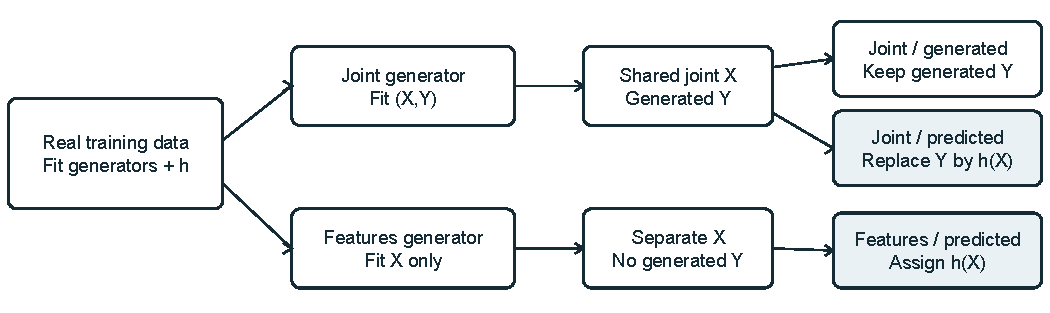
\includegraphics[width=\columnwidth]{figures/constructions.pdf}
\caption{The three synthetic-table constructions. Shaded constructions use
targets predicted by a labeler $h$ trained on real training data.}
\label{fig:constructions}
\end{figure}

\subsection{Learning the Target Predictor}
We use three labelers: a random forest (RF)~\citep{breiman2001rf},
gradient-boosted trees (XGB)~\citep{chen2016xgboost}, and a feed-forward
neural network (DNN). Each is fitted to the real training partition only.
For classification, $h$ outputs a hard class decision; for regression, it
outputs a point prediction. Labelers are not selected on test performance;
all three are reported.

\subsection{Synthetic-only and Mixed Training}
Each synthetic table is evaluated in two regimes. \emph{Synthetic-only}
training uses the synthetic rows alone. \emph{Mixed} training concatenates
all real training rows with all 100,000 synthetic rows; it is not a fixed
50/50 mixture. A real-only model trained on the real training partition is
the reference for both regimes.

\section{Experimental Setup}
\subsection{Real-data Benchmark}
The benchmark contains five classification tasks (Adult, Census KDD,
Covertype, MNIST12, and MNIST28) and two regression tasks (News and
California Housing), each with experiment seeds 42 and 43. Rows are
partitioned before any fitted preprocessing. Identical feature rows are kept
in the same partition, the split random state is shared across experiment
seeds, and a rare-class rule can move a feature group into training, so
realized partition sizes vary slightly by task. Encodings, scaling,
generators, and labelers are fitted on training data only.

CTGAN, TVAE, and TabDDPM are trained for 500 epochs with batch size 500, and
each generator samples 100,000 rows. TabDDPM is run as an unconditional
joint or features-only model under the same protocol; this is not a
replication of its original conditional classification benchmark.
Downstream utility is measured with dataset-specific neural networks
trained with batch size 128, learning rate $10^{-3}$, at most 100 epochs,
and patience 30. Scaling and encodings are fitted on real training
features even for synthetic-only training.

\paragraph{Checkpoint selection.} Each downstream model's checkpoint is the
earliest epoch with the best real-development score within its completed
training history: binary F1 for Adult, macro F1 for the other
classification tasks, and $R^2$ for regression. We report these
validation-best checkpoints because development loss can disagree sharply
with the reported F1 on imbalanced tasks. Regression checkpoints are the
same under both rules. Section~\ref{sec:sensitivity} repeats the analysis
with loss-selected checkpoints.

In total, each task contributes $2$ seeds $\times\,(1 + 2\times 21)$
evaluations: one real-only model and 21 synthetic constructions
($3$ generators $\times\,[1 + 2\times 3]$) in each training regime, or
602 evaluations overall.

\subsection{Construction of the Simulated Datasets}
The simulated benchmark separates prediction from recovery of
the original joint distribution. Each dataset has independent training
and test draws of 10,000 rows, and each synthetic table has 10,000 rows.
Experiment seeds are 42 and 43. CTGAN and TVAE use 300 epochs and batch
size 500. The seven datasets comprise three mixed continuous/categorical
distributions and four categorical Bayesian networks.

\subsubsection{Gaussian, Grid, and Ring}
Each row contains two continuous features $X=(X_0,X_1)$, a binary feature
$C$, and a binary target $Y$. The three datasets differ only in the
distribution of $X$, and each coordinate of $X$ has mean zero and unit
variance. Gaussian draws $X\sim\mathcal N(0,I_2)$. Grid and Ring draw a mode
center $M$, add isotropic noise, and rescale:
\begin{equation}
 X=\frac{M+\tau Z}{\sqrt{v+\tau^2}},\qquad Z\sim\mathcal N(0,I_2),\quad \tau=0.2.
\end{equation}
For Grid, each coordinate of $M$ is uniform on $\{-4,-2,0,2,4\}$, giving 25
equally likely modes and $v=8$. For Ring,
$M=(\cos(\pi K/4),\sin(\pi K/4))$ with $K$ uniform on
$\{0,\dots,7\}$, giving eight modes on a circle and $v=1/2$; its two
coordinates are dependent. Here $v$ is the variance of one coordinate of
$M$, so the scaling is the known population standard deviation.

$C$ and $Y$ follow the same rule in all three datasets. Writing
$S=2C-1\in\{-1,+1\}$ and $\sigma$ for the logistic function,
\begin{equation}
 P(S=s\mid X)=\sigma(2sX_0X_1),
\end{equation}
\begin{equation}
 h^*(X,S)=\mathbf 1\{X_1+(1+3S/4)\,X_0>0\},
\end{equation}
\begin{equation}
 P\big(Y=h^*(X,S)\mid X,S\big)=0.9 .
\end{equation}
Thus $S$ is a noisy indicator of whether $X_0$ and $X_1$ share a sign, and
the Bayes decision boundary is a line through the origin whose slope,
$-1/4$ or $-7/4$, is selected by $S$ (Figure~\ref{fig:simulated-construction}).
The observed target flips $h^*$ independently with probability $0.1$, so
the Bayes accuracy is $0.9$, and for any classifier $h$,
$P(h\neq Y)=0.1+0.8\,P(h\neq h^*)$. Agreement with $h^*$ therefore measures
how well a classifier learned the decision rule, without the irreducible
label noise. Every feature affects the target, and $C$ is independent of each
coordinate of $X$ alone.

\begin{figure*}[t]
\centering
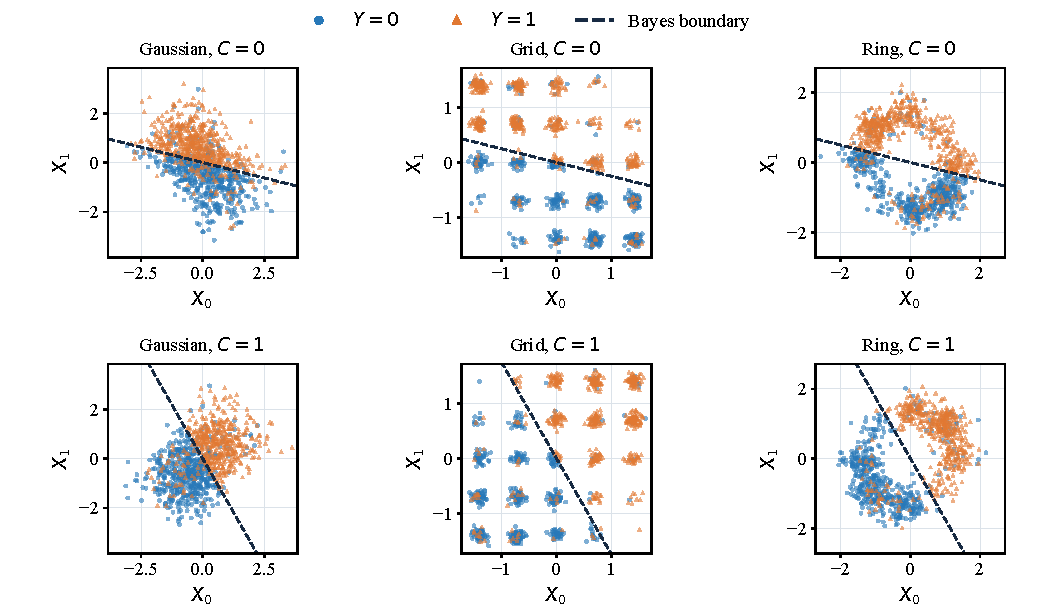
\includegraphics[width=\textwidth]{figures/simulated_construction.pdf}
\caption{Gaussian, Grid, and Ring, conditioned on the binary feature $C$.
Points are original-process rows; circles denote $Y=0$ and triangles
denote $Y=1$. Dashed lines show the Bayes decision boundary. Each dataset
is illustrated with 2,000 saved rows (seed 7), independent of the
benchmark's 10,000-row draws with seeds 42 and 43.}
\label{fig:simulated-construction}
\end{figure*}

\subsubsection{Categorical Bayesian Networks}
Asia, Alarm, Child, and Insurance use the packaged graphs and their
original conditional probability tables. We sample ancestrally from each
network, designate one node as the target (Table~\ref{tab:simulated-schema}),
and observe every other node as a feature. State codes are categorical,
not ordinal. No additional label noise is introduced. Figure~\ref{fig:asia}
shows Asia as an example. Oracle posteriors are computed by enumerating
the target states with the other nodes observed. Bayes accuracy is
estimated by averaging the maximum posterior over independent test features.
\begin{table}[t]
\centering
{\small
\begin{tabular}{lrlr}
\toprule
Network & Features & Target & States \\
\midrule
Asia & 7 & \texttt{dysp} & 2 \\
Alarm & 36 & \texttt{BP} & 3 \\
Child & 19 & \texttt{Disease} & 6 \\
Insurance & 26 & \texttt{Accident} & 4 \\
\bottomrule
\end{tabular}
}
\caption{Categorical Bayesian-network datasets. Every non-target node is observed. Original conditional probability tables define each joint distribution.}
\label{tab:simulated-schema}
\end{table}

\begin{figure}[t]
\centering
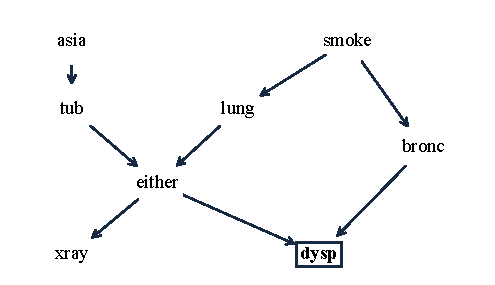
\includegraphics[width=\columnwidth]{figures/asia_graph.pdf}
\caption{The Asia network. The boxed node, \texttt{dysp}, is the target;
all other nodes are observed features. Arrows and conditional probability
tables define the original joint distribution used to sample rows.}
\label{fig:asia}
\end{figure}

\subsection{Evaluation Metrics}
Real-data classification tables report binary and macro F1 for Adult and
Census KDD, macro F1 for Covertype, and accuracy for MNIST12 and MNIST28.
Statistical contrasts use macro F1 for every classification task.
Regression tables report $R^2$ and $D^2$ absolute error, where $D^2$ is one
minus the test MAE divided by the MAE of the constant test-median
predictor. Both are unscaled, and higher is better.

\paragraph{Simulated-data protocol and metrics.} The simulated benchmark has
one training regime: each training table (the 10,000 original training
rows for \emph{real only}, or 10,000 generated or relabeled rows) is used
alone. A fresh DNN with two 64-unit hidden layers is trained on it and
evaluated on the same independent 10,000-row original test set. This is the
analogue of synthetic-only training on real data; there is no mixed regime.
The main tables use RF, XGB, and DNN labelers, as for real data. For each
training table $T$ we report four scores. The first two measure prediction; higher is
better.
\emph{Accuracy} is measured against the observed test targets.
\emph{$h^*$ agreement} is the fraction of test rows on which the downstream
DNN predicts the Bayes decision $h^*(x)$; it removes the irreducible label
noise from the comparison. The two remaining scores measure fidelity to
the true joint density $p$ of all columns, from opposite directions:
\begin{equation}
 L_{\rm syn}=\frac1{|T|}\sum_{z\in T}\log p(z),
\end{equation}
\begin{equation}
 L_{\rm test}=\frac1{|D_{\rm test}|}\sum_{z\in D_{\rm test}}\log\hat q_T(z).
\end{equation}
$L_{\rm syn}$ scores the \emph{synthetic} rows under the \emph{true}
density: it asks whether they are plausible, and, like precision, it can
be raised by concentrating rows in high-density regions while missing
others. $L_{\rm test}$ fits a density $\hat q_T$ from a fixed family to the
training table and scores \emph{real} test rows under it: like recall, it
penalizes modes and variation that $T$ lacks. It is a refit proxy, not a
generator likelihood. The fixed families mirror each true model: Gaussian or
Gaussian-mixture features, a logistic model for $C$, a flip-rate model for
$Y$, and, for the networks, the true graph with conditional probability
tables re-estimated under a Dirichlet$(1/2)$ prior. Network scores use
$\log(p+10^{-8})$ on the full joint probability, because some rows have
probability zero.

\paragraph{Statistical analysis.} The independent unit is a dataset. For
each classification task we average over seeds (which share held-out
partitions), labelers, and generators with equal weight, then fit a
two-level repeated-measures ANOVA, $\mathrm{score}\sim\mathrm{dataset}+
\mathrm{condition}$, giving $F(1,4)$. The relabeled arm averages joint and
X-only relabeling; generated-target baselines enter once. Holm correction
covers the four primary tests (two contrasts $\times$ two regimes), and a
separate Holm family covers the twelve generator-specific tests. With two
regression tasks, regression tests have $F(1,1)$ and are treated as
descriptive.

\section{Results on Real Data}
\begin{table*}[p]
\centering
\footnotesize
\setlength{\tabcolsep}{6pt}
\begin{tabular}{@{}lrrrrrrr@{}}
\toprule
\textbf{Method} & \multicolumn{2}{c}{\textbf{Adult}} & \multicolumn{2}{c}{\textbf{Census KDD}} & \multicolumn{1}{c}{\textbf{Covertype}} & \multicolumn{1}{c}{\textbf{MNIST12}} & \multicolumn{1}{c}{\textbf{MNIST28}} \\
\cmidrule(lr){2-3}\cmidrule(lr){4-5}\cmidrule(lr){6-6}\cmidrule(lr){7-7}\cmidrule(lr){8-8}
 & Bin.\ F1 & Mac.\ F1 & Bin.\ F1 & Mac.\ F1 & Mac.\ F1 & Acc. & Acc. \\
\midrule
Real only & 67.88 & 79.25 & \underline{55.21} & 75.63 & 52.58 & \textbf{95.57} & \textbf{97.92} \\
\midrule
CTGAN, generated $Y$ & 63.40 & 76.51 & 47.42 & 71.05 & 46.48 & 54.00 & 57.54 \\
CTGAN joint + RF & 66.15 & 78.38 & 50.91 & 73.76 & 61.81 & 90.06 & 87.56 \\
CTGAN joint + XGB & 66.69 & 78.63 & 54.69 & 75.69 & 64.68 & 91.39 & 88.61 \\
CTGAN joint + DNN & \textbf{69.34} & 79.39 & 54.08 & 75.47 & 72.80 & 91.93 & 92.02 \\
CTGAN X-only + RF & 66.66 & 78.68 & 52.75 & 74.66 & 62.25 & 88.85 & 88.08 \\
CTGAN X-only + XGB & 67.38 & 78.95 & 54.24 & 75.45 & 65.07 & 90.42 & 88.91 \\
CTGAN X-only + DNN & 69.26 & \textbf{79.50} & 54.40 & 75.74 & 71.26 & 90.93 & 92.24 \\
\addlinespace
TVAE, generated $Y$ & 61.36 & 75.26 & 47.00 & 71.21 & 47.27 & 92.97 & 94.19 \\
TVAE joint + RF & 66.14 & 78.29 & 49.64 & 72.90 & 58.09 & 93.06 & 94.76 \\
TVAE joint + XGB & 67.61 & 78.97 & 52.04 & 74.33 & 58.76 & \underline{94.20} & 96.00 \\
TVAE joint + DNN & 69.10 & \underline{79.40} & 53.04 & 74.94 & 68.50 & 93.95 & 95.96 \\
TVAE X-only + RF & 67.20 & 78.90 & 48.53 & 72.21 & 55.43 & 92.81 & 94.87 \\
TVAE X-only + XGB & 67.81 & 79.18 & 49.92 & 73.13 & 55.31 & 94.11 & \underline{96.05} \\
TVAE X-only + DNN & \underline{69.31} & 79.33 & 52.85 & 74.79 & 67.18 & 93.73 & 96.00 \\
\addlinespace
TabDDPM, generated $Y$ & 66.22$^{\dagger}$ & 78.49$^{\dagger}$ & 46.81 & 70.95 & 52.33 & 73.30 & 43.16 \\
TabDDPM joint + RF & 67.32$^{\dagger}$ & 79.06$^{\dagger}$ & 50.93 & 74.01 & 67.77 & 66.65 & 57.97 \\
TabDDPM joint + XGB & 68.32$^{\dagger}$ & 79.56$^{\dagger}$ & 53.82 & 75.56 & 68.10 & 54.04 & 49.96 \\
TabDDPM joint + DNN & 69.19$^{\dagger}$ & 79.31$^{\dagger}$ & 53.76 & 75.53 & \underline{75.68} & 22.00 & 15.76 \\
TabDDPM X-only + RF & 66.56$^{\dagger}$ & 78.62$^{\dagger}$ & 52.92 & 74.92 & 65.88 & 75.03 & 36.29 \\
TabDDPM X-only + XGB & 67.57$^{\dagger}$ & 79.10$^{\dagger}$ & \textbf{55.62} & \textbf{76.36} & 68.92 & 66.21 & 30.64 \\
TabDDPM X-only + DNN & 69.12$^{\dagger}$ & 79.36$^{\dagger}$ & 54.48 & \underline{75.86} & \textbf{75.88} & 32.28 & 16.49 \\
\bottomrule
\end{tabular}
\caption{Classification, synthetic-only training (validation-best checkpoints; \%). Test means over seeds 42/43; higher is better. Joint: features from the full-table generator with $Y$ replaced by the named labeler; X-only: a separate features-only generator followed by the labeler. Bold/underline: best/second-best distinct displayed value, including real only. $\dagger$: Adult TabDDPM has an unresolved historical generator-source caveat and is excluded from ranking. MNIST12 TVAE retains a documented exact held-out feature-collision caveat; MNIST12 TabDDPM shows a diagnosed generated-input shift that is retained as a result.}
\label{tab:valbest-synthetic}
\end{table*}

\begin{table*}[p]
\centering
\footnotesize
\setlength{\tabcolsep}{6pt}
\begin{tabular}{@{}lrrrrrrr@{}}
\toprule
\textbf{Method} & \multicolumn{2}{c}{\textbf{Adult}} & \multicolumn{2}{c}{\textbf{Census KDD}} & \multicolumn{1}{c}{\textbf{Covertype}} & \multicolumn{1}{c}{\textbf{MNIST12}} & \multicolumn{1}{c}{\textbf{MNIST28}} \\
\cmidrule(lr){2-3}\cmidrule(lr){4-5}\cmidrule(lr){6-6}\cmidrule(lr){7-7}\cmidrule(lr){8-8}
 & Bin.\ F1 & Mac.\ F1 & Bin.\ F1 & Mac.\ F1 & Mac.\ F1 & Acc. & Acc. \\
\midrule
Real only & 67.88 & 79.25 & 55.21 & 75.63 & 52.58 & \textbf{95.57} & \textbf{97.92} \\
\midrule
CTGAN, generated $Y$ & 65.51 & 77.72 & 44.69 & 68.42 & 51.55 & 71.89 & 92.77 \\
CTGAN joint + RF & 66.77 & 78.60 & 56.61 & 76.85 & 56.63 & 92.95 & 95.70 \\
CTGAN joint + XGB & 67.84 & 79.31 & 56.83 & 76.94 & 62.46 & 94.07 & 96.63 \\
CTGAN joint + DNN & 69.38 & 79.22 & 56.80 & 76.94 & \underline{76.72} & 94.01 & 96.33 \\
CTGAN X-only + RF & 67.82 & 79.26 & 55.82 & 76.47 & 57.03 & 92.83 & 95.78 \\
CTGAN X-only + XGB & 68.50 & \textbf{79.55} & 56.98 & 76.98 & 62.24 & 93.94 & 96.24 \\
CTGAN X-only + DNN & \underline{69.42} & 79.37 & 56.99 & 77.10 & 76.08 & 94.03 & 96.41 \\
\addlinespace
TVAE, generated $Y$ & 61.66 & 75.74 & 55.39 & 75.86 & 49.41 & 94.40 & 96.37 \\
TVAE joint + RF & 66.00 & 78.28 & 55.63 & 76.24 & 59.94 & 93.91 & 95.96 \\
TVAE joint + XGB & 67.53 & 79.00 & \textbf{57.80} & \underline{77.40} & 61.43 & \underline{94.93} & \underline{96.88} \\
TVAE joint + DNN & 68.85 & 79.17 & 57.00 & 77.09 & 74.75 & 94.75 & 96.69 \\
TVAE X-only + RF & 66.87 & 78.82 & 56.15 & 76.56 & 56.30 & 93.94 & 96.02 \\
TVAE X-only + XGB & 67.75 & 79.14 & \underline{57.74} & \textbf{77.42} & 56.66 & 94.89 & \underline{96.88} \\
TVAE X-only + DNN & \textbf{69.46} & \underline{79.50} & 57.36 & 77.30 & 74.53 & 94.72 & 96.77 \\
\addlinespace
TabDDPM, generated $Y$ & 65.36$^{\dagger}$ & 78.07$^{\dagger}$ & 45.20 & 69.16 & 49.08 & 88.84 & 88.74 \\
TabDDPM joint + RF & 66.75$^{\dagger}$ & 78.77$^{\dagger}$ & 55.08 & 76.13 & 66.53 & 79.83 & 93.13 \\
TabDDPM joint + XGB & 68.63$^{\dagger}$ & 79.71$^{\dagger}$ & 56.95 & 77.07 & 67.08 & 91.06 & 93.02 \\
TabDDPM joint + DNN & 69.17$^{\dagger}$ & 79.28$^{\dagger}$ & 55.79 & 76.51 & 76.51 & 51.61 & 46.28 \\
TabDDPM X-only + RF & 67.13$^{\dagger}$ & 78.99$^{\dagger}$ & 55.25 & 76.22 & 64.67 & 91.51 & 93.34 \\
TabDDPM X-only + XGB & 67.95$^{\dagger}$ & 79.30$^{\dagger}$ & 57.12 & 77.13 & 68.13 & 92.70 & 64.15 \\
TabDDPM X-only + DNN & 69.27$^{\dagger}$ & 79.53$^{\dagger}$ & 56.56 & 76.97 & \textbf{77.44} & 65.79 & 48.95 \\
\bottomrule
\end{tabular}
\caption{Classification, real + synthetic training (all real training rows plus 100,000 synthetic rows; \%). Checkpoints, notation, highlighting, and caveats follow Table~\ref{tab:valbest-synthetic}.}
\label{tab:valbest-mix}
\end{table*}

\begin{table*}[p]
\centering
\small
\setlength{\tabcolsep}{6pt}
\begin{tabular}{@{}lrrrrrrrr@{}}
\toprule
 & \multicolumn{4}{c}{\textbf{Synthetic only}} & \multicolumn{4}{c}{\textbf{Real + synthetic}} \\
\cmidrule(lr){2-5}\cmidrule(lr){6-9}
\textbf{Method} & \multicolumn{2}{c}{\textbf{News}} & \multicolumn{2}{c}{\textbf{Housing}} & \multicolumn{2}{c}{\textbf{News}} & \multicolumn{2}{c}{\textbf{Housing}} \\
\cmidrule(lr){2-3}\cmidrule(lr){4-5}\cmidrule(lr){6-7}\cmidrule(lr){8-9}
 & $R^2$ & $D^2$ & $R^2$ & $D^2$ & $R^2$ & $D^2$ & $R^2$ & $D^2$ \\
\midrule
Real only & -0.029 & -0.044 & 0.512 & 0.282 & -0.029 & -0.044 & 0.512 & 0.282 \\
\midrule
CTGAN, generated $Y$ & -0.019 & \textbf{0.015} & 0.631 & 0.414 & -0.017 & \underline{0.024} & 0.636 & 0.419 \\
CTGAN joint + RF & -0.003 & -0.006 & 0.790 & 0.599 & -0.002 & 0.010 & 0.786 & 0.591 \\
CTGAN joint + XGB & -0.007 & 0.007 & 0.817 & \textbf{0.627} & -0.002 & 0.009 & \underline{0.813} & \textbf{0.623} \\
CTGAN joint + DNN & 0.001 & \underline{0.008} & 0.800 & 0.609 & \underline{0.001} & 0.017 & 0.787 & 0.609 \\
CTGAN X-only + RF & 0.000 & -0.001 & 0.790 & 0.586 & -0.002 & 0.008 & 0.782 & 0.588 \\
CTGAN X-only + XGB & 0.000 & -0.010 & 0.819 & 0.621 & \textbf{0.002} & 0.000 & 0.810 & \underline{0.616} \\
CTGAN X-only + DNN & 0.002 & 0.007 & 0.804 & 0.607 & -0.001 & 0.020 & 0.803 & 0.608 \\
\addlinespace
TVAE, generated $Y$ & -0.027 & 0.005 & 0.714 & 0.505 & -0.022 & \textbf{0.036} & 0.700 & 0.503 \\
TVAE joint + RF & 0.000 & -0.006 & 0.785 & 0.581 & -0.001 & 0.005 & 0.776 & 0.570 \\
TVAE joint + XGB & -0.002 & -0.011 & \underline{0.821} & \textbf{0.627} & -0.001 & 0.011 & 0.762 & 0.615 \\
TVAE joint + DNN & \underline{0.008} & -0.028 & 0.746 & 0.594 & \underline{0.001} & 0.011 & 0.798 & 0.605 \\
TVAE X-only + RF & 0.003 & -0.003 & 0.779 & 0.573 & \underline{0.001} & 0.002 & 0.761 & 0.555 \\
TVAE X-only + XGB & 0.002 & -0.032 & 0.817 & \underline{0.622} & -0.001 & 0.009 & 0.800 & 0.606 \\
TVAE X-only + DNN & \textbf{0.010} & -0.021 & 0.758 & 0.606 & \underline{0.001} & 0.009 & 0.787 & 0.601 \\
\addlinespace
TabDDPM, generated $Y$ & -0.028 & -0.026 & 0.791 & 0.587 & \textbf{0.002} & -0.074 & 0.787 & 0.573 \\
TabDDPM joint + RF & 0.001 & -0.009 & 0.793 & 0.589 & -0.002 & 0.003 & 0.789 & 0.582 \\
TabDDPM joint + XGB & 0.000 & -0.022 & \textbf{0.823} & 0.618 & \underline{0.001} & -0.007 & \textbf{0.816} & 0.613 \\
TabDDPM joint + DNN & -0.007 & -0.014 & 0.797 & 0.594 & -0.009 & -0.008 & 0.793 & 0.589 \\
TabDDPM X-only + RF & 0.000 & -0.002 & 0.791 & 0.586 & -0.002 & 0.009 & 0.786 & 0.578 \\
TabDDPM X-only + XGB & 0.004 & -0.026 & \textbf{0.823} & 0.620 & -0.001 & -0.008 & \textbf{0.816} & 0.609 \\
TabDDPM X-only + DNN & -0.004 & -0.051 & 0.799 & 0.601 & -0.004 & -0.035 & 0.796 & 0.593 \\
\bottomrule
\end{tabular}
\caption{Regression, both training regimes. Test means over seeds 42/43; higher is better. $D^2$ is absolute-error skill relative to the constant test-median predictor; both metrics are unscaled. Construction names and highlighting follow Table~\ref{tab:valbest-synthetic}.}
\label{tab:valbest-regression}
\end{table*}

\begin{table}[t]
\centering
\small
\setlength{\tabcolsep}{2pt}
\begin{tabular}{@{}lrrrr@{}}
\toprule
Contrast & $\Delta$ & 95\% CI & $p$ & $p_{\rm Holm}$ \\
\midrule
\multicolumn{5}{@{}l}{\emph{Synthetic only}} \\
Relabeled $-$ generated & +7.36 & [+0.1, +14.7] & 0.049 & 0.196 \\
Joint $-$ X-only & +0.46 & [-3.0, +3.9] & 0.726 & 1.000 \\
\quad CTGAN relab.\ $-$ gen. & +20.57 & [-1.4, +42.6] & 0.060 & 0.724 \\
\quad CTGAN joint $-$ X-only & +0.07 & [-0.7, +0.8] & 0.802 & 1.000 \\
\quad TVAE relab.\ $-$ gen. & +4.32 & [-2.1, +10.7] & 0.133 & 1.000 \\
\quad TVAE joint $-$ X-only & +0.60 & [-0.8, +2.0] & 0.289 & 1.000 \\
\quad TabDDPM relab.\ $-$ gen. & -2.83 & [-23.7, +18.0] & 0.726 & 1.000 \\
\quad TabDDPM joint $-$ X-only & +0.72 & [-10.2, +11.7] & 0.864 & 1.000 \\
\midrule
\multicolumn{5}{@{}l}{\emph{Real + synthetic}} \\
Relabeled $-$ generated & +4.73 & [-4.6, +14.1] & 0.233 & 0.700 \\
Joint $-$ X-only & +0.15 & [-2.6, +2.9] & 0.888 & 1.000 \\
\quad CTGAN relab.\ $-$ gen. & +10.14 & [-1.0, +21.2] & 0.064 & 0.724 \\
\quad CTGAN joint $-$ X-only & +0.00 & [-0.2, +0.3] & 0.966 & 1.000 \\
\quad TVAE relab.\ $-$ gen. & +3.84 & [-3.7, +11.4] & 0.232 & 1.000 \\
\quad TVAE joint $-$ X-only & +0.46 & [-1.2, +2.1] & 0.487 & 1.000 \\
\quad TabDDPM relab.\ $-$ gen. & +0.20 & [-18.6, +19.0] & 0.978 & 1.000 \\
\quad TabDDPM joint $-$ X-only & -0.02 & [-8.1, +8.0] & 0.994 & 1.000 \\
\bottomrule
\end{tabular}
\caption{Repeated-measures ANOVA on five classification tasks, $F(1,4)$, macro F1 in percentage points. Seeds, labelers (RF/XGB/DNN), and generators are averaged with equal weight before inference; the dataset is the unit. Relabeled averages both feature sources. Pooled rows: Holm over the four primary tests; indented generator rows: Holm over 12 tests. Intervals are unadjusted.}
\label{tab:anova}
\end{table}

\begin{table}[t]
\centering
\small
\setlength{\tabcolsep}{3pt}
\begin{tabular}{@{}llrrrr@{}}
\toprule
& & \multicolumn{2}{c}{Relabeled $-$ gen.} & \multicolumn{2}{c}{Joint $-$ X-only} \\
\cmidrule(lr){3-4}\cmidrule(lr){5-6}
Checkpoint & Tasks & Synth. & Mix & Synth. & Mix \\
\midrule
Dev.\ metric & All five & +7.36 & +4.73 & +0.46 & +0.15 \\
Dev.\ metric & No Adult & +8.63 & +5.41 & +0.60 & +0.24 \\
Dev.\ metric & No MNIST12 & +7.85 & +4.93 & +1.35 & +0.94 \\
Dev.\ metric & Neither & +9.71 & +5.92 & +1.83 & +1.33 \\
\addlinespace
Dev.\ loss & All five & +7.48 & +4.46 & -0.49 & +0.55 \\
Dev.\ loss & No Adult & +8.71 & +5.20 & -0.50 & +0.86 \\
Dev.\ loss & No MNIST12 & +8.29 & +4.59 & +0.34 & +1.50 \\
Dev.\ loss & Neither & +10.21 & +5.63 & +0.60 & +2.23 \\
\bottomrule
\end{tabular}
\caption{Sensitivity of the two primary contrasts (macro F1, percentage points) to the checkpoint rule and to excluding caveated tasks. No contrast passes Holm correction in any cohort.}
\label{tab:sensitivity}
\end{table}

Tables~\ref{tab:valbest-synthetic}--\ref{tab:valbest-regression} report every
construction, and Figure~\ref{fig:effects} summarizes the relabeling effect
by task and generator.

\subsection{Does Replacing the Targets Help?}
Averaged over generators and labelers, predicted targets improve
synthetic-only macro F1 on all five classification tasks: by 2.3 points on
Adult, 3.7 on Census KDD, 17.0 on Covertype, 5.4 on MNIST12, and 8.4 on
MNIST28. The pooled gain is 7.36 points (95\% CI $[0.1, 14.7]$, $p=0.049$),
which does not survive Holm correction ($p_{\rm Holm}=0.196$;
Table~\ref{tab:anova}). In mixed training, the pooled gain is 4.73 points
($p=0.233$); four tasks improve and MNIST28 declines by 4.3 points.

The effect depends strongly on the generator. CTGAN benefits most: its
generated targets are poor on MNIST12 and MNIST28 (54.0\% and 57.5\%
synthetic-only accuracy), and relabeling raises them to roughly 88--92\%.
Its generator-specific gain is 20.6 points in synthetic-only training and
10.1 in mixed training ($p=0.060$ and $0.064$, unadjusted). TVAE's
generated targets are already more consistent with its features, and its
gains are smaller (4.3 and 3.8 points). TabDDPM shows no average benefit
($-2.8$ and $+0.2$ points). Its Covertype and Census KDD results improve
with relabeling, but on MNIST12 and MNIST28 most relabeled tables, and
all DNN-labeled tables, are much worse than its generated-target baseline
(e.g., 22.0\% versus 73.3\% synthetic-only accuracy for joint DNN
relabeling on MNIST12). A diagnostic check found that TabDDPM's generated
pixel distribution differs from the real one while retaining transferable
digit structure: a model trained on its generated targets reaches 73\% real
test accuracy, but real-trained labelers disagree with 78--88\% of the
generated targets and assign many rows to a single digit. Relabeling
thereby overwrites a useful generated association. A labeler trained on
real data is only as reliable as the overlap between generated and real
features.

Covertype stands out. Several relabeled constructions exceed the real-only
reference by more than 20 macro-F1 points, in both regimes. The
real-only downstream network reaches 52.6\% macro F1, and the relabeled
DNN tables reach 67--78\%. We read this as evidence that, on this task,
training the downstream network on a large table labeled by a strong
labeler acts as distillation of that labeler, rather than as evidence that
the synthetic features are better than the real ones.
% TODO: report the labelers' own test macro F1 on Covertype to support this.

For regression (Table~\ref{tab:valbest-regression}), relabeling improves Housing substantially: generated-target
$R^2$ ranges from 0.631 (CTGAN) to 0.791 (TabDDPM), and relabeled
constructions reach 0.75--0.82, all above the real-only reference of 0.512.
News has essentially no predictable signal under this protocol: every
construction, including real-only training, has $R^2$ near zero, and
relabeling does not change that conclusion. With only two regression tasks,
the $F(1,1)$ tests are uninformative (synthetic-only $\Delta R^2=0.055$,
$p=0.32$).

\begin{figure*}[t]
\centering
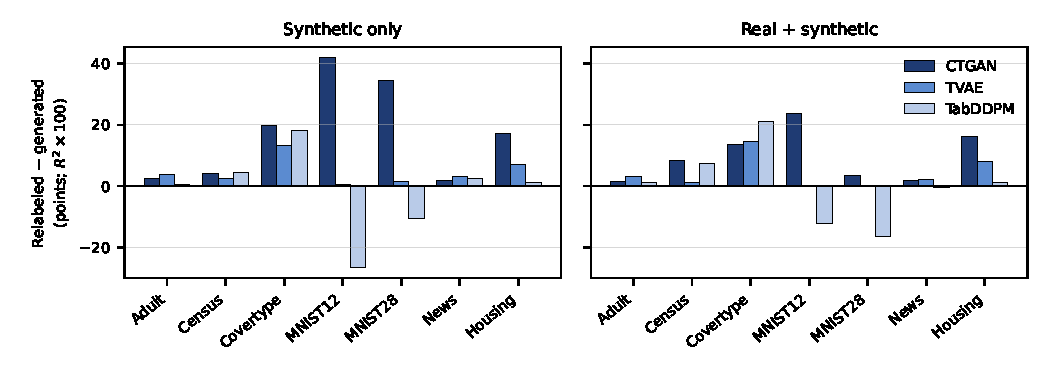
\includegraphics[width=0.85\textwidth]{figures/valbest_effects.pdf}
\caption{Relabeled minus generated, by task and generator, averaged over
seeds, RF/XGB/DNN labelers, and both feature sources. Classification uses
macro F1 (percentage points); regression uses $R^2\times100$. The Adult
TabDDPM bar carries the generator-source caveat of
Table~\ref{tab:valbest-synthetic}.}
\label{fig:effects}
\end{figure*}

\subsection{Does the Generator Need to Model the Target?}
Joint and features-only relabeling perform similarly. The pooled
joint-minus-X-only difference is $+0.46$ macro-F1 points in synthetic-only
training (95\% CI $[-3.0, 3.9]$) and $+0.15$ in mixed training
($[-2.6, 2.9]$). Task-level differences change sign: joint generation is
better on MNIST28 ($+4.6$) and Covertype ($+1.0$) and worse on MNIST12
($-3.1$), with Adult and Census KDD within 0.2 points. Housing and News
show differences below 0.002 in $R^2$. The intervals are wide, so these
results do not establish equivalence; they indicate that any benefit of
modeling $Y$ during feature generation is small compared with the effect of
the target assignment itself.


\subsection{Sensitivity}
\label{sec:sensitivity}
Table~\ref{tab:sensitivity} repeats the primary contrasts with
loss-selected checkpoints and after excluding the two caveated tasks
(Adult, because of the TabDDPM caveat, and MNIST12, because of TVAE feature
collisions). The relabeling gain is stable in sign and size, between 7.4
and 10.2 points in synthetic-only training and between 4.5 and 5.9 in
mixed training. The joint-minus-X-only estimate changes sign between
checkpoint rules and remains small. No contrast passes Holm correction in
any cohort.

\section{Results on Simulated Data}
\begin{table*}[p]
\centering
\small
\setlength{\tabcolsep}{7pt}
\begin{tabular}{@{}lrrrrrrr@{}}
\toprule
\textbf{Method} & \textbf{Gaussian} & \textbf{Grid} & \textbf{Ring} & \textbf{Asia} & \textbf{Alarm} & \textbf{Child} & \textbf{Insurance} \\
\midrule
\multicolumn{8}{@{}l}{\textbf{(a) Test accuracy (\%)}} \\
\addlinespace[2pt]
Bayes accuracy & 90.00 & 90.00 & 90.00 & 85.32 & 82.13 & 89.09 & 95.46 \\
\midrule
Real only & \underline{89.42} & \underline{90.09} & \textbf{89.75} & 85.76 & 80.91 & 87.48 & 94.67 \\
\midrule
CTGAN, generated $Y$ & 77.72 & 83.53 & 85.98 & 85.67 & 55.31 & 79.74 & 88.93 \\
CTGAN joint + RF & \underline{89.42} & 90.01 & 89.54 & 85.67 & 80.55 & \textbf{87.98} & 94.99 \\
CTGAN joint + XGB & 89.40 & 89.85 & 89.64 & \textbf{85.78} & \textbf{81.63} & 87.88 & \textbf{95.06} \\
CTGAN joint + DNN & 89.33 & 89.95 & 89.66 & 85.76 & 80.78 & 87.66 & 94.83 \\
CTGAN X-only + RF & 89.31 & \textbf{90.11} & 89.59 & 85.67 & 80.88 & 87.64 & 94.97 \\
CTGAN X-only + XGB & 89.31 & 90.03 & 89.55 & \textbf{85.78} & 81.53 & 87.88 & \underline{95.03} \\
CTGAN X-only + DNN & 89.39 & 89.62 & \underline{89.72} & 85.76 & 80.75 & 87.89 & 95.01 \\
\addlinespace
TVAE, generated $Y$ & 86.39 & 89.01 & 89.00 & 85.30 & 77.03 & 85.10 & 91.68 \\
TVAE joint + RF & \textbf{89.52} & 89.84 & 89.55 & 85.71 & 79.88 & 87.59 & 94.30 \\
TVAE joint + XGB & 89.10 & 89.96 & 89.69 & \underline{85.77} & \underline{81.62} & 87.77 & 94.08 \\
TVAE joint + DNN & 89.30 & 89.62 & 89.68 & 85.56 & 80.82 & 87.78 & 94.05 \\
TVAE X-only + RF & 89.06 & 87.95 & 89.68 & 85.71 & 79.99 & 87.54 & 94.49 \\
TVAE X-only + XGB & 88.78 & 87.94 & 89.66 & \underline{85.77} & 81.53 & \underline{87.94} & 94.74 \\
TVAE X-only + DNN & 88.93 & 87.89 & 89.66 & 85.75 & 80.81 & 87.66 & 94.40 \\
\midrule
\multicolumn{8}{@{}l}{\textbf{(b) Agreement with the Bayes rule $h^*$ (\%)}} \\
\addlinespace[2pt]
Real only & 99.28 & \underline{99.71} & \textbf{99.56} & \underline{99.98} & 95.24 & 95.41 & 97.25 \\
\midrule
CTGAN, generated $Y$ & 84.63 & 91.76 & 94.82 & 99.71 & 59.19 & 84.59 & 91.66 \\
CTGAN joint + RF & 99.29 & 99.58 & 99.30 & 99.88 & 94.71 & 96.05 & \underline{98.12} \\
CTGAN joint + XGB & \underline{99.30} & 99.39 & 99.44 & \textbf{100.00} & \textbf{97.40} & \underline{96.17} & 97.85 \\
CTGAN joint + DNN & 99.21 & 99.50 & 99.47 & \underline{99.98} & 94.94 & 95.80 & 97.78 \\
CTGAN X-only + RF & 99.21 & \textbf{99.77} & 99.39 & 99.89 & 94.62 & 95.87 & \textbf{98.14} \\
CTGAN X-only + XGB & 99.22 & \underline{99.71} & 99.32 & \textbf{100.00} & 97.02 & 96.09 & 97.95 \\
CTGAN X-only + DNN & 99.25 & 99.19 & \underline{99.53} & \underline{99.98} & 94.97 & 95.94 & 97.78 \\
\addlinespace
TVAE, generated $Y$ & 95.60 & 98.33 & 98.62 & 99.30 & 87.76 & 91.40 & 93.73 \\
TVAE joint + RF & \textbf{99.39} & 99.43 & 99.33 & 99.91 & 93.57 & 95.75 & 97.31 \\
TVAE joint + XGB & 98.91 & 99.58 & 99.51 & \textbf{100.00} & \underline{97.20} & 96.14 & 96.99 \\
TVAE joint + DNN & 99.13 & 99.13 & 99.48 & 99.72 & 95.09 & 95.59 & 96.81 \\
TVAE X-only + RF & 98.95 & 97.07 & 99.47 & 99.90 & 93.34 & 95.88 & 97.65 \\
TVAE X-only + XGB & 98.61 & 97.08 & 99.45 & \textbf{100.00} & 97.09 & \textbf{96.61} & 97.84 \\
TVAE X-only + DNN & 98.75 & 97.00 & 99.44 & \underline{99.98} & 95.72 & 95.93 & 97.36 \\
\bottomrule
\end{tabular}
\caption{Simulated data, synthetic-only training: prediction. Each training table (10,000 rows) trains a fresh downstream DNN that is scored on the same independent 10,000-row original test set; means over seeds 42/43. (a) Accuracy against the observed test targets; the Bayes accuracy is 90\% for the three mixed datasets and the mean maximum oracle posterior for the Bayesian networks. (b) Fraction of test rows on which the DNN predicts the Bayes decision $h^*(x)$. Construction names follow Table~\ref{tab:valbest-synthetic}. Bold/underline: best/second-best displayed value, including real only.}
\label{tab:sim-prediction}
\end{table*}

\begin{table*}[p]
\centering
\small
\setlength{\tabcolsep}{7pt}
\begin{tabular}{@{}lrrrrrrr@{}}
\toprule
\textbf{Method} & \textbf{Gaussian} & \textbf{Grid} & \textbf{Ring} & \textbf{Asia} & \textbf{Alarm} & \textbf{Child} & \textbf{Insurance} \\
\midrule
\multicolumn{8}{@{}l}{\textbf{(a) $L_{\rm syn}$: mean $\log p$ of the training rows under the true distribution}} \\
\addlinespace[2pt]
Real only & -3.69 & -1.55 & -3.00 & -2.24 & -10.24 & -12.06 & -12.91 \\
\midrule
CTGAN, generated $Y$ & -4.56 & -2.53 & -4.60 & -3.72 & -15.61 & -13.89 & -16.83 \\
CTGAN joint + RF & -4.01 & -2.12 & -4.05 & -3.52 & -15.10 & -13.46 & -16.69 \\
CTGAN joint + XGB & -3.99 & -2.10 & -4.03 & -3.52 & -15.07 & -13.44 & -16.68 \\
CTGAN joint + DNN & -3.98 & -2.09 & -4.01 & -3.52 & -15.08 & -13.45 & -16.69 \\
CTGAN X-only + RF & -4.03 & -2.03 & -4.09 & -3.46 & -15.24 & -13.27 & -16.84 \\
CTGAN X-only + XGB & -4.01 & -2.01 & -4.07 & -3.45 & -15.22 & -13.24 & -16.84 \\
CTGAN X-only + DNN & -4.00 & -2.00 & -4.04 & -3.46 & -15.23 & -13.25 & -16.84 \\
\addlinespace
TVAE, generated $Y$ & -3.60 & -1.31 & -3.17 & -2.29 & -11.22 & -12.43 & -14.06 \\
TVAE joint + RF & -3.36 & -1.19 & -2.90 & -2.02 & -10.95 & -12.13 & -13.97 \\
TVAE joint + XGB & -3.35 & -1.16 & -2.88 & -2.02 & -10.91 & -12.10 & -13.97 \\
TVAE joint + DNN & -3.34 & -1.16 & -2.87 & -2.02 & -10.92 & -12.11 & -13.98 \\
TVAE X-only + RF & -3.05 & -1.58 & -2.88 & -1.99 & -11.01 & -12.37 & -14.03 \\
TVAE X-only + XGB & -3.04 & -1.55 & -2.86 & -1.99 & -10.97 & -12.33 & -14.03 \\
TVAE X-only + DNN & -3.02 & -1.54 & -2.86 & -1.99 & -10.98 & -12.34 & -14.04 \\
\midrule
\multicolumn{8}{@{}l}{\textbf{(b) $L_{\rm test}$: mean $\log q$ of real test rows, $q$ refitted to the training table}} \\
\addlinespace[2pt]
Real only & -3.68 & -1.55 & -3.00 & -2.22 & -10.31 & -12.04 & -12.90 \\
\midrule
CTGAN, generated $Y$ & -4.07 & -1.97 & -3.65 & -2.45 & -12.95 & -12.78 & -14.88 \\
CTGAN joint + RF & -3.94 & -1.99 & -3.56 & -3.23 & -12.73 & -12.69 & -14.77 \\
CTGAN joint + XGB & -3.98 & -2.05 & -3.59 & -3.29 & -12.82 & -12.71 & -14.77 \\
CTGAN joint + DNN & -4.02 & -2.20 & -3.66 & -2.96 & -12.70 & -12.70 & -14.77 \\
CTGAN X-only + RF & -3.95 & -1.95 & -3.54 & -3.23 & -12.69 & -12.66 & -14.86 \\
CTGAN X-only + XGB & -3.97 & -2.00 & -3.56 & -3.26 & -12.78 & -12.69 & -14.86 \\
CTGAN X-only + DNN & -3.99 & -2.10 & -3.62 & -2.96 & -12.66 & -12.67 & -14.87 \\
\addlinespace
TVAE, generated $Y$ & -3.76 & -1.60 & -3.08 & -2.24 & -10.78 & -12.24 & -13.55 \\
TVAE joint + RF & -3.84 & -1.70 & -3.17 & -3.09 & -10.87 & -12.20 & -13.54 \\
TVAE joint + XGB & -3.89 & -1.92 & -3.25 & -3.10 & -11.09 & -12.23 & -13.54 \\
TVAE joint + DNN & -3.91 & -1.99 & -3.31 & -3.04 & -10.98 & -12.22 & -13.53 \\
TVAE X-only + RF & -4.21 & -3.67 & -3.22 & -3.09 & -10.82 & -12.23 & -13.41 \\
TVAE X-only + XGB & -4.25 & -3.85 & -3.31 & -3.10 & -11.07 & -12.26 & -13.41 \\
TVAE X-only + DNN & -4.29 & -4.15 & -3.37 & -2.98 & -10.92 & -12.25 & -13.40 \\
\bottomrule
\end{tabular}
\caption{Simulated data: fidelity of each training table to the true joint distribution $p$ of $(X, C, Y)$ or of all network nodes. Both are mean log densities, but they answer different questions. $L_{\rm syn}$ asks whether the synthetic rows are plausible under $p$ and rewards rows concentrated in high-density regions even if modes are missed, so values above real only signal concentration rather than better fidelity. $L_{\rm test}$ fits a fixed density family to the table and asks whether it explains real test rows, so it penalizes missing modes and missing target noise. Real only gives the reference value for each task. Means over seeds 42/43; each task has its own log-density scale, so values are not comparable across tasks. Bayesian-network scores use $\log(p+10^{-8})$ on the full joint probability.}
\label{tab:sim-fidelity}
\end{table*}

Tables~\ref{tab:sim-prediction} and~\ref{tab:sim-fidelity} use the same
layout as the real-data tables. All entries use synthetic-only training
and a downstream DNN; only the construction of the training table changes.

\subsection{Predictive Utility and Bayes Agreement}
Generated targets are the weak point of both generators. CTGAN's generated
tables reach only 55.3\% accuracy on Alarm and 77.7\% on Gaussian, against
real-only values of 80.9\% and 89.4\%. TVAE's generated targets are better
but still trail real only on every task. Replacing the targets
closes nearly all of this gap. With either joint or X-only features and
any of the three labelers, accuracy is within about one point of real-only
training on every task except TVAE X-only on Grid (about 88\% against
90.1\%). Averaged over generators, labelers, and seeds, joint relabeling
raises accuracy by between 0.2 points (Asia) and 14.7 points (Alarm), and
$h^*$ agreement by between 0.4 and 22.0 points. Agreement gains exceed
accuracy gains because for the mixed datasets each point of disagreement
with $h^*$ costs only 0.8 points of accuracy. On Alarm, Child, and
Insurance, several relabeled tables agree with $h^*$ more often than
real-only training does: the labeler, trained on the same 10,000 real rows,
passes on its estimate of the decision rule without the label noise.
Accuracy on Asia slightly exceeds the estimated Bayes accuracy because
both are finite-sample estimates.

\subsection{Joint-distribution Fidelity}
The fidelity scores tell a different story (Table~\ref{tab:sim-fidelity}).
Real-only training tables have the highest $L_{\rm test}$ on every task.
Relabeling raises $L_{\rm syn}$ on every task, by 0.12 to 0.43 nats on
average for joint relabeling, because hard labels move each row's target
to its most probable value given the features. For TVAE, relabeled tables
even exceed the real-only $L_{\rm syn}$ on Gaussian, Grid, Ring, and Asia.
That is concentration, not better fidelity. $L_{\rm test}$ moves the other
way on four tasks: joint relabeling lowers it on Gaussian, Grid, Ring, and
Asia, because a density refitted to noise-free targets assigns low
probability to real test rows whose target disagrees with $h^*$. It is
essentially unchanged on Alarm and slightly higher on Child and Insurance. On Asia,
relabeling barely changes accuracy (0.2 points) yet lowers $L_{\rm test}$ by
0.77 nats. Figure~\ref{fig:oracle} shows these changes for each generator
and labeler. A table can therefore be more useful for prediction while
being a worse sample of the original joint distribution.

\begin{figure*}[t]
\centering
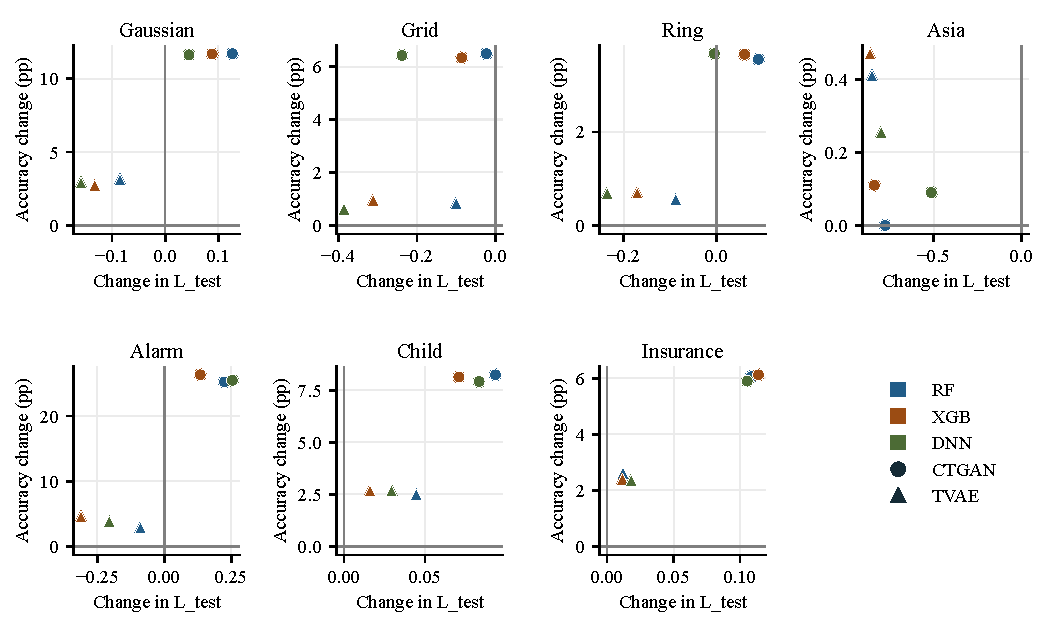
\includegraphics[width=0.8\textwidth]{figures/oracle_tradeoff.pdf}
\caption{Simulated data: change in $L_{\rm test}$ (horizontal) against
change in accuracy (vertical, percentage points) from joint relabeling,
relative to generated targets. Shape: generator; color: labeler. Each point
averages two seeds; no trend is fitted.}
\label{fig:oracle}
\end{figure*}

\section{Discussion}
\subsection{When Does Target Replacement Help?}
Relabeling helps most when the generator's conditional $P(\widetilde Y\mid
\widetilde X)$ is poor, as for CTGAN on the MNIST tasks and for all
generators on Covertype, and when the generated features remain within the
region where the real-trained labeler is reliable. It can hurt when the
generated features are shifted, as for TabDDPM on MNIST. A practical check
is therefore not the labeler's real-data accuracy alone, but whether its
predictions on generated features agree with the generator's own targets
or with a held-out feature-shift diagnostic. We did not choose labelers by
test score; DNN labelers are often, but not always, the strongest.

\subsection{Does the Generator Need to Model the Target?}
After relabeling, joint and features-only generators gave similar utility.
Practitioners who intend to relabel may therefore fit the generator to $X$
alone without a measurable loss, at least for the generators and tasks we
study. Conversely, there is little evidence that fitting the joint model
yields better feature distributions for downstream prediction.

\section{Limitations}
The real-data inference has five classification tasks, so power is low and
task effects are heterogeneous; seeds share real-data partitions and do not
represent new datasets. MNIST12 and MNIST28 are related tasks. Adult
TabDDPM results carry an unresolved historical generator-source caveat. The
MNIST12 TVAE data retain a documented exact held-out feature-collision
caveat, and MNIST12 TabDDPM retains a diagnosed generated-input shift.
Validation-best checkpoints are selected within the original training
histories and were chosen after loss-based selection had been examined; the
loss-selected analysis gives similar conclusions. TabDDPM is run
unconditionally, unlike its original classification protocol. Hard
relabeling does not reproduce target noise, and density-refit scores depend
on the specified estimators. Credit and the naive-Bayes and PCA/GMM
labelers are outside the reported, balanced comparison.

\section{Conclusion}
Target assignment is a separate design decision in synthetic tabular data.
Replacing generated targets with predictions from a labeler trained on real
data improved average downstream utility, by large margins for CTGAN and
modest ones for TVAE, but not for TabDDPM, and the pooled gain was not
statistically established across five tasks. Whether the generator modeled
the target mattered little once targets were predicted. On simulated
data, the same replacement moved predictions closer to the Bayes
rule while making the synthetic table a less faithful sample of the
original joint distribution. Evaluations of synthetic data should report
how targets were assigned and should not treat predictive utility as a
measure of distributional fidelity.

\bibliography{references}
\end{document}
